% MD5 ("frastoca") = d4e02542ff15febf3ca60b1e048d23db
%
%  untitled
%
%  Created by Andrés Alessandro León Baldelli.
%  Copyright (c) 2015  All rights reserved.
%
\documentclass[]{article}

% Use utf-8 encoding for foreign characters
\usepackage[utf8]{inputenc}
\usepackage{pmboxdraw}

\usepackage[lined]{algorithm2e}
\usepackage[top=1cm, left=1.5cm, right=1.5cm, bottom=1cm]{geometry}
% pygments
\usepackage{fancyvrb}
\usepackage{color}
\usepackage[english]{babel}
\usepackage{datetime}
% end pygments
\usepackage{geometry}
\usepackage{eurosym}
\usepackage[backend=biber,style=numeric,natbib=true,giveninits=true,url=false,doi=false,isbn=false,maxnames=5]{biblatex}
% \addbibresource{biblio.bib}
%\AtEveryBibitem{  \clearfield{day}  \clearfield{month}  \clearfield{endday}  \clearfield{endmonth}}

\usepackage[pdftex,pdfauthor={Andres A Leon Baldelli},pdftitle={},pdfsubject={},pdfkeywords={},pdfproducer={Latex with hyperref},pdfcreator={pdflatex}]{hyperref}


% Running Headers and footers
%\usepackage{fancyhdr}

% Multipart figures
%\usepackage{subfigure}

% More symbols
\usepackage{amsmath}
\usepackage{amssymb}
\usepackage{latexsym}
\usepackage{multicol}

% Surround parts of graphics with box
\usepackage{boxedminipage}
% Package for including code in the document
\usepackage{listings}

% If you want to generate a toc for each chapter (use with book)
\usepackage{minitoc}

% This is now the recommended way for checking for PDFLaTeX:
\usepackage{ifpdf}

% 
\newenvironment{system}% 
{\left\lbrace\begin{array}{@{}l@{}}}% 
{\end{array}\right.} 

\usepackage[shortlabels,inline]{enumitem}
\setlist[itemize,1]{label={\textbullet}}
\setlist{noitemsep}
\setlist[1]{labelindent=\parindent,
  itemsep=0ex,
  leftmargin=1em,
  labelwidth=10em
  }
\setlist*[enumerate,1]{%
  label=(\roman*),
}
\newlist{inlinelist}{itemize*}{1}
\setlist[inlinelist,1]{%
  label={},
  before=\unskip{: }, itemjoin={{; }}, itemjoin*={{ et }}
}
\newcommand{\proj}{\emph{FUCK HSBC}}
\input{/Users/kumiori/Documents/WIP/tex_macros/incl_macro_gen.tex}
\ifpdf
\usepackage{graphicx}
% \fi
\title{
\vspace{-2em}
\textbf{``Class Stability'' 50/50} - 
Project: \textbf{\proj}~  }
\author{  
\emph{IM3}\footnote{}~,
IM2\footnote{},  
IM1\footnote{}
}

\date{\vspace{-5em}}

\begin{document}

\ifpdf
\DeclareGraphicsExtensions{.pdf, .jpg, .tif}
\else
\DeclareGraphicsExtensions{.eps, .jpg}
\fi

\maketitle


\begin{center}
\Large{}






\end{center}

\noindent\emph{\textbf{Keywords:} 
}

\medskip

\textbf{Abstract}
Fuck HSBC, and the banking system \emph{as a consequence}.
\section{Context}
With help from the automated language \emph{graph transversal} ride. A fast one.
We analyse a few classes of damage models.
For fun and !profit.



\begin{figure}[htbp]
  \centering
  \includegraphics[width=.8\textwidth]{../figures/generic_class_analyser.png}
  \caption{class analysis}
  \label{fig:class-analyser}
\end{figure}

\section*{ATk = LS = JJK}
\newcommand{\ilen}{\ell}
State = $y:=(u, \alpha)$
Material parameters:
{k: k, E0: 1, w1: w1, $\ilen$: $\ilen$, L: L} are variables.


\begin{verbatim}
  atk = DefaultDamage(state, _matpar)


ana = ModelAnalysis(atk)
_crit = sp.diff(atk.energy(state), a).subs({u: _u0, a: _a0}).simplify()
_crit
\end{verbatim}


\begin{equation}
  \label{eqn:mod-crit}
  % \left\{
    u{\left(x \right)} = \frac{t x}{L} \qquad
  \alpha{\left(x \right)} = 
  \begin{cases} 
      -- \frac{t}{L \sqrt{w_{1}}} & \text{for}: t \geq \\ 
      0 & \text{otherwise}
  \end{cases}
  % \right\}
\end{equation}

critical load

\begin{equation}
  \label{eqn:mod-crit-load}
  % \left\{ u{\left(x \right)} : \frac{t x}{L}, \  
  % \alpha{\left(x \right)} : \begin{cases} -- \frac{t}{L \sqrt{w_{1}}} & \text{for}\: t \geq \0 & \text{otherwise} \end{cases}\right\}
  \left[ - L \sqrt{w_{1}}, \  L \sqrt{w_{1}}\right]
\end{equation}




\begin{Verbatim}
  sp.diff(atk.energy(state), \alpha) \
    .subs({u: _u0, \alpha: \alpha}) \
    .simplify()
\end{Verbatim}

\begin{equation}
  \label{eqn:mod-eqdiff}
  \frac{w_{1} \alpha^{2}{\left(x \right)} + 2 w_{1} \alpha{\left(x \right)} + w_{1} - \frac{t^{2}}{L^{2}}}{\alpha^{2}{\left(x \right)} + 2 \alpha{\left(x \right)} + 1}
  =0
\end{equation}

\begin{figure}[htbp]
  \centering
  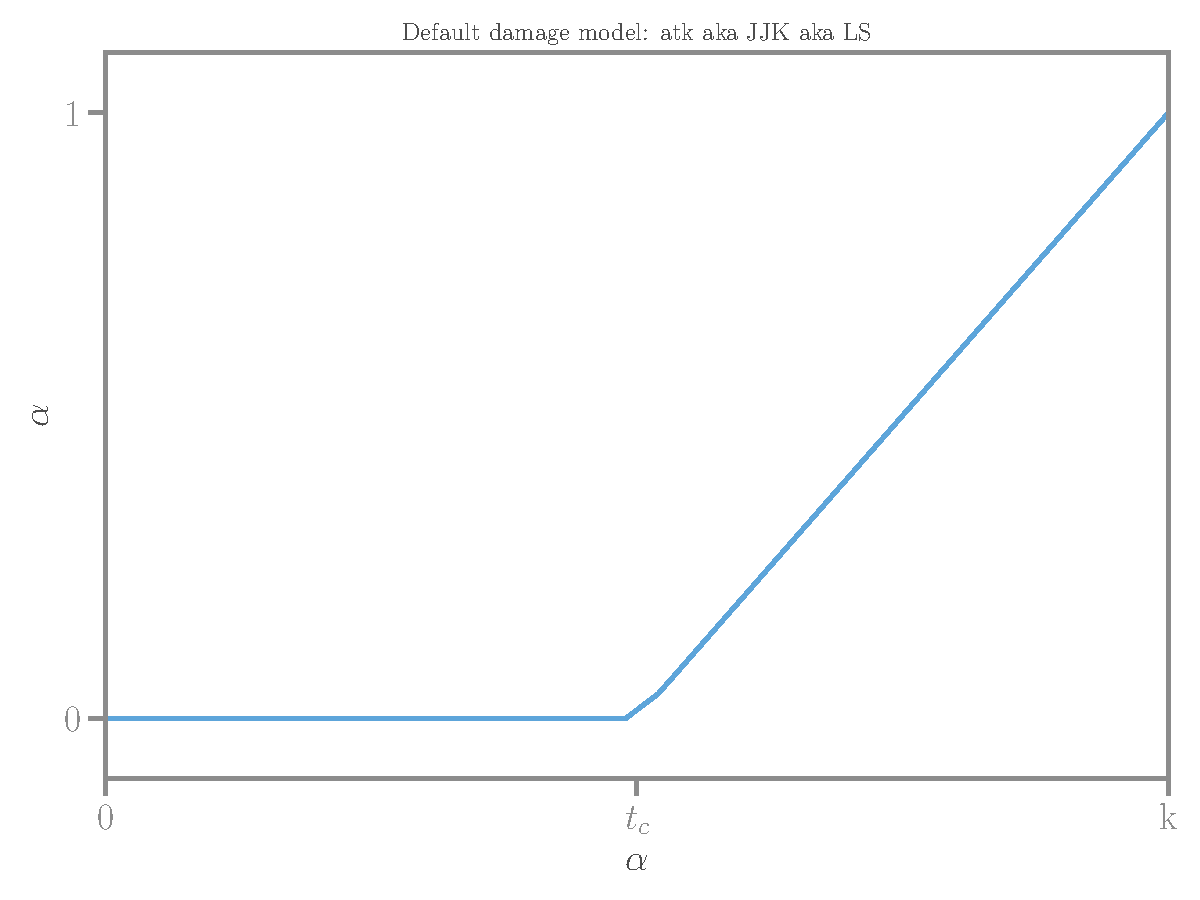
\includegraphics[width=.33\textheight]{../figures/atk-alpha-homog.pdf}
  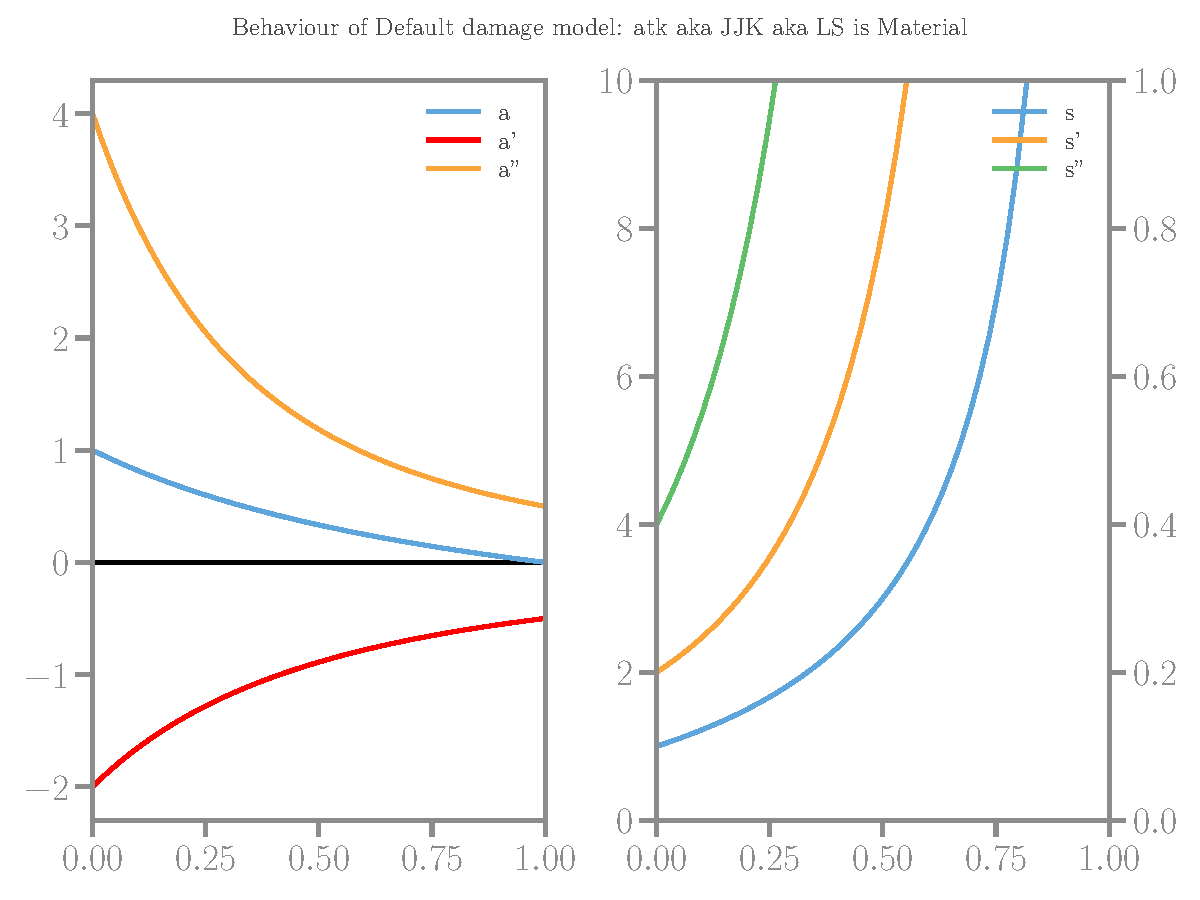
\includegraphics[width=.33\textheight]{../figures/atk-model.pdf}
  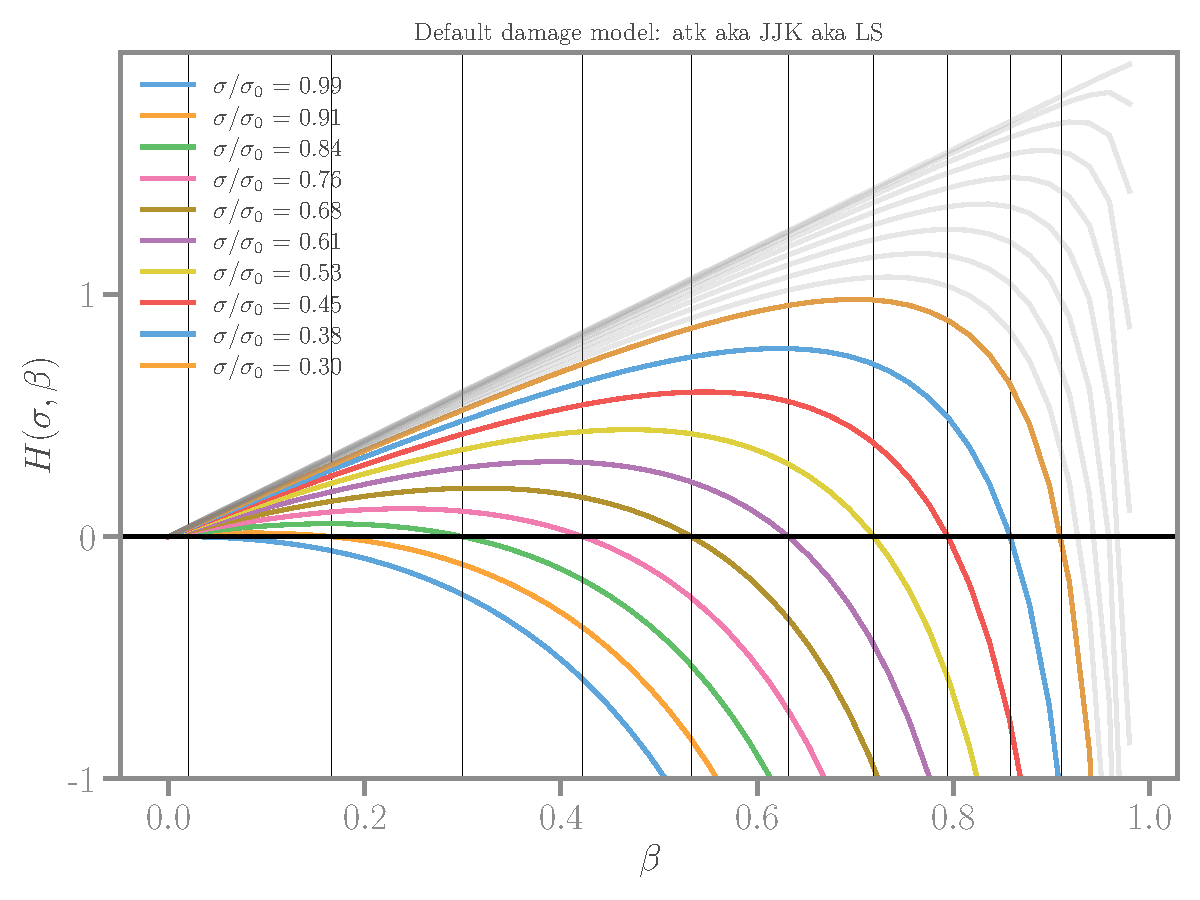
\includegraphics[width=.33\textheight]{../figures/atk-Hbeta.pdf}
  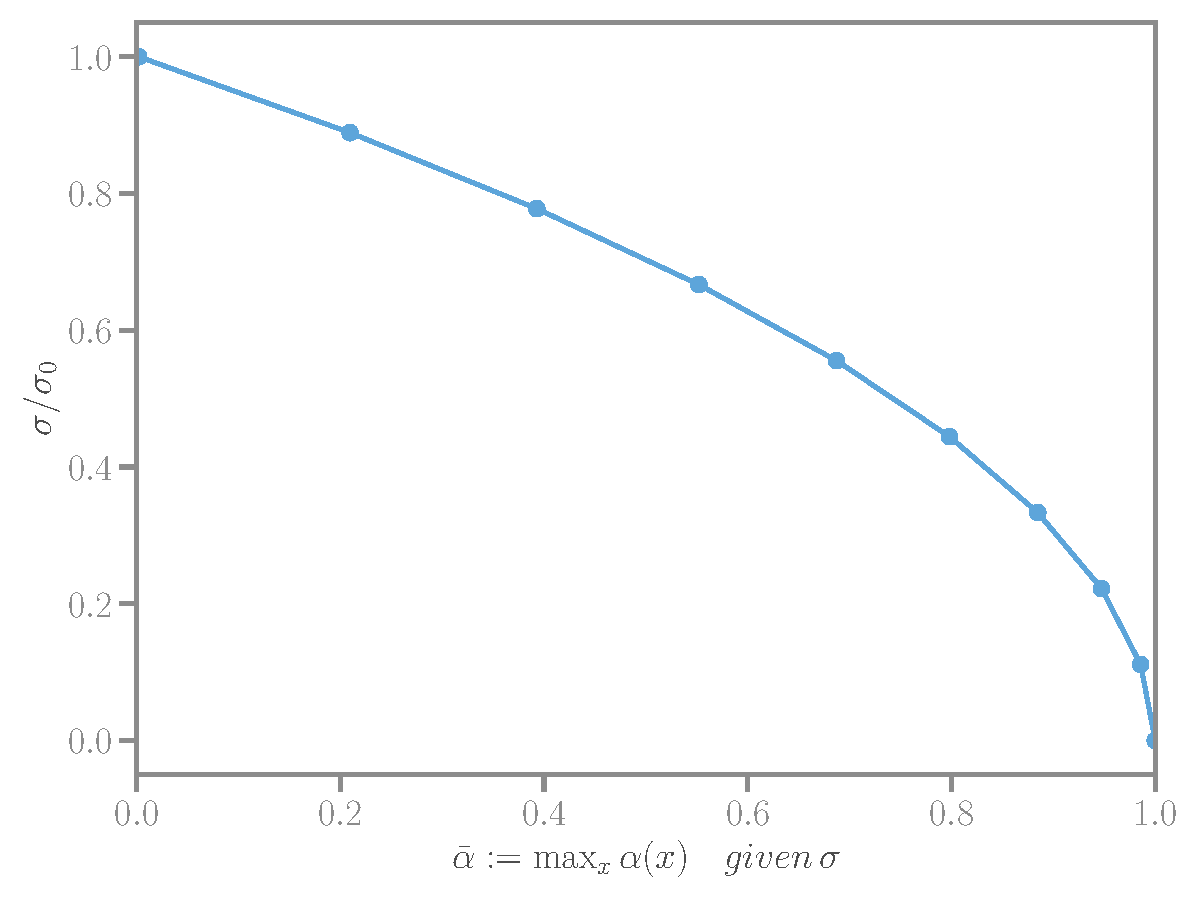
\includegraphics[width=.33\textheight]{../figures/atk-maxalpha.pdf}
  \caption{class analysis}
  \label{fig:class-analyser}
\end{figure}
\section*{ATn}
\subsection*{$n=2$}


matpar = ${n: 1, E0: 1, w1: 1, \ilen: \ilen}$



\begin{Verbatim}
  ana.criterion(), ana.critical_load(), ana._homogeneous_alpha()  
\end{Verbatim}



\begin{equation}
  \label{eqn:mod-criterion}
  0=- \frac{1.0 E_{0} t^{2}}{L^{2}} + 1
\end{equation}

critical load $t_c = L \sqrt{\frac{1}{E_{0}}}$

\begin{equation}
  \label{eqn:mod-energy}
E(y)  =  \int_0^L
\ilen^{2} \left(\frac{d}{d x} \alpha{\left(x \right)}\right)^{2} + \frac{1}{2} E_0\left(1 - \alpha{\left(x \right)}\right)^{2} \left(\frac{d}{d x} u{\left(x \right)}\right)^{2} + \alpha{\left(x \right)}
\end{equation}


homogeneous state

\begin{equation}
  \label{eqn:mod-homogeneous}
  \alpha_t =
  \begin{cases}
    1 - \frac{L^{2}}{E_{0} t^{2}} & \text{for}\: t \geq 1 \\
    0 & \text{otherwise} \end{cases}
\end{equation}



\begin{figure}[htbp]
  \centering
  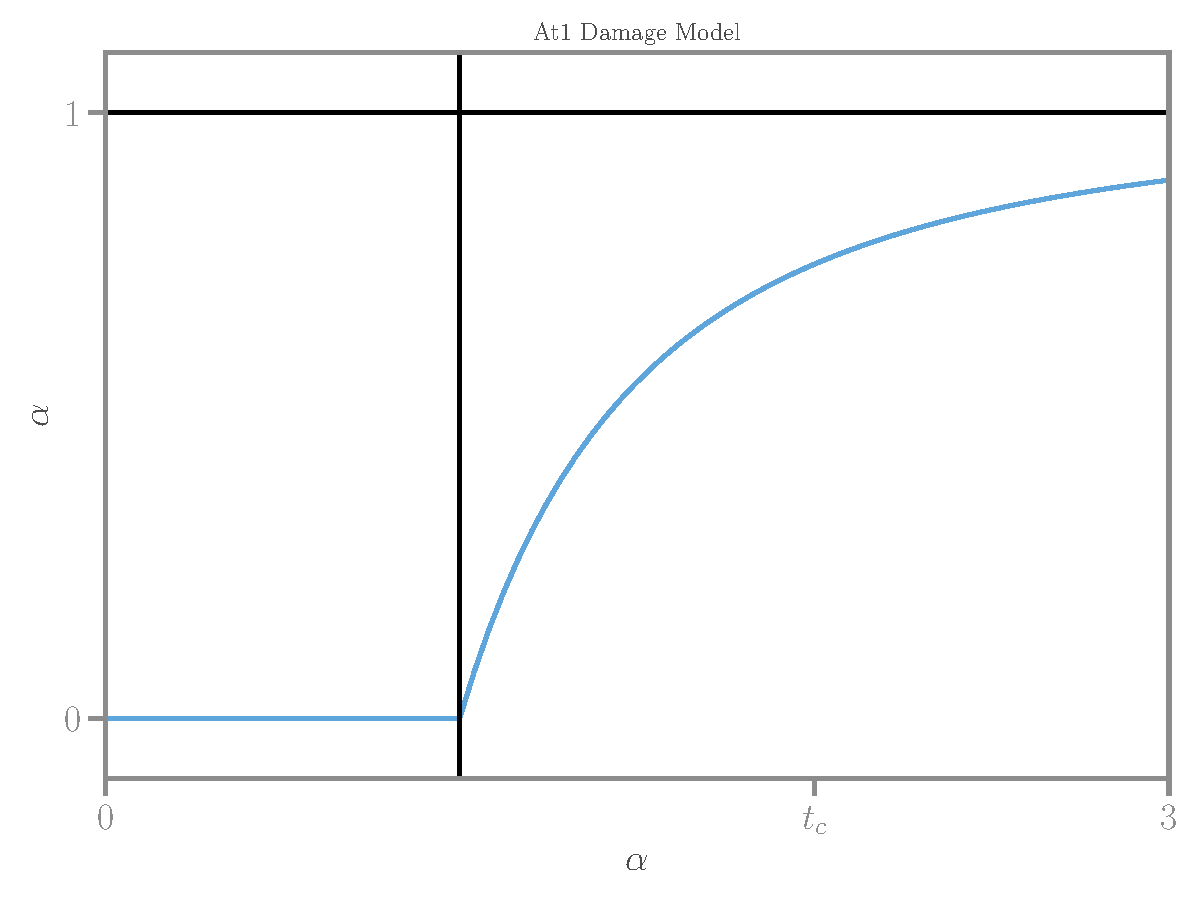
\includegraphics[width=.33\textheight]{../figures/at1-alpha-homog.pdf}
  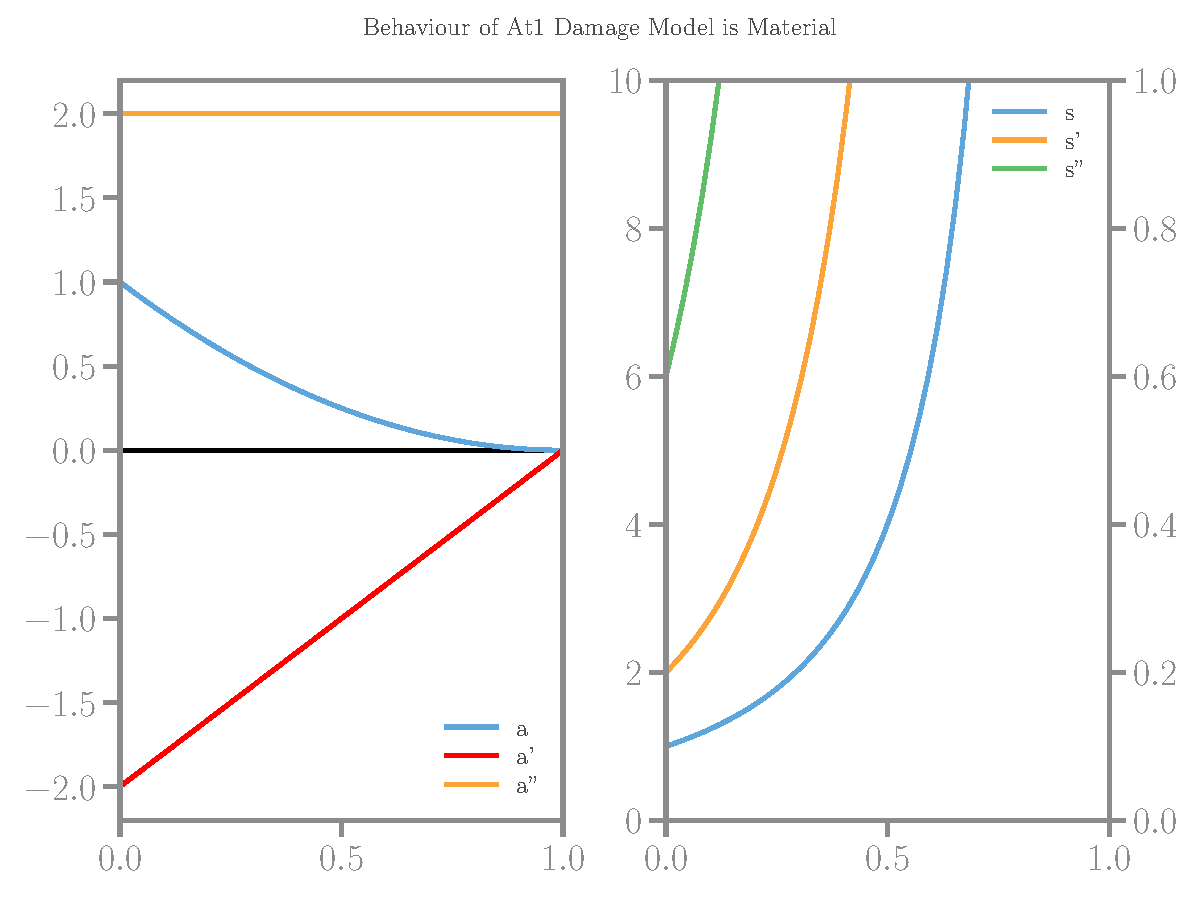
\includegraphics[width=.33\textheight]{../figures/at1-model.pdf}
  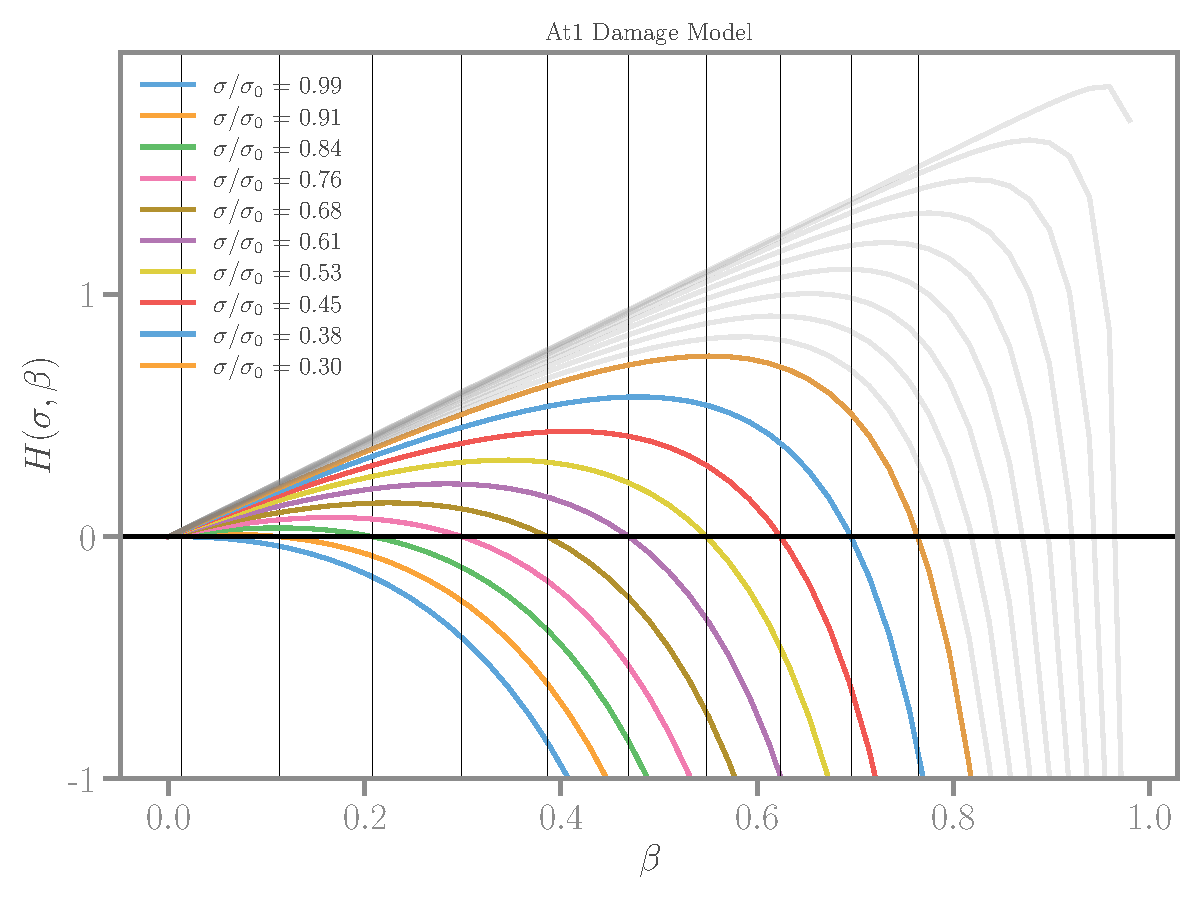
\includegraphics[width=.33\textheight]{../figures/at1-Hbeta.pdf}
  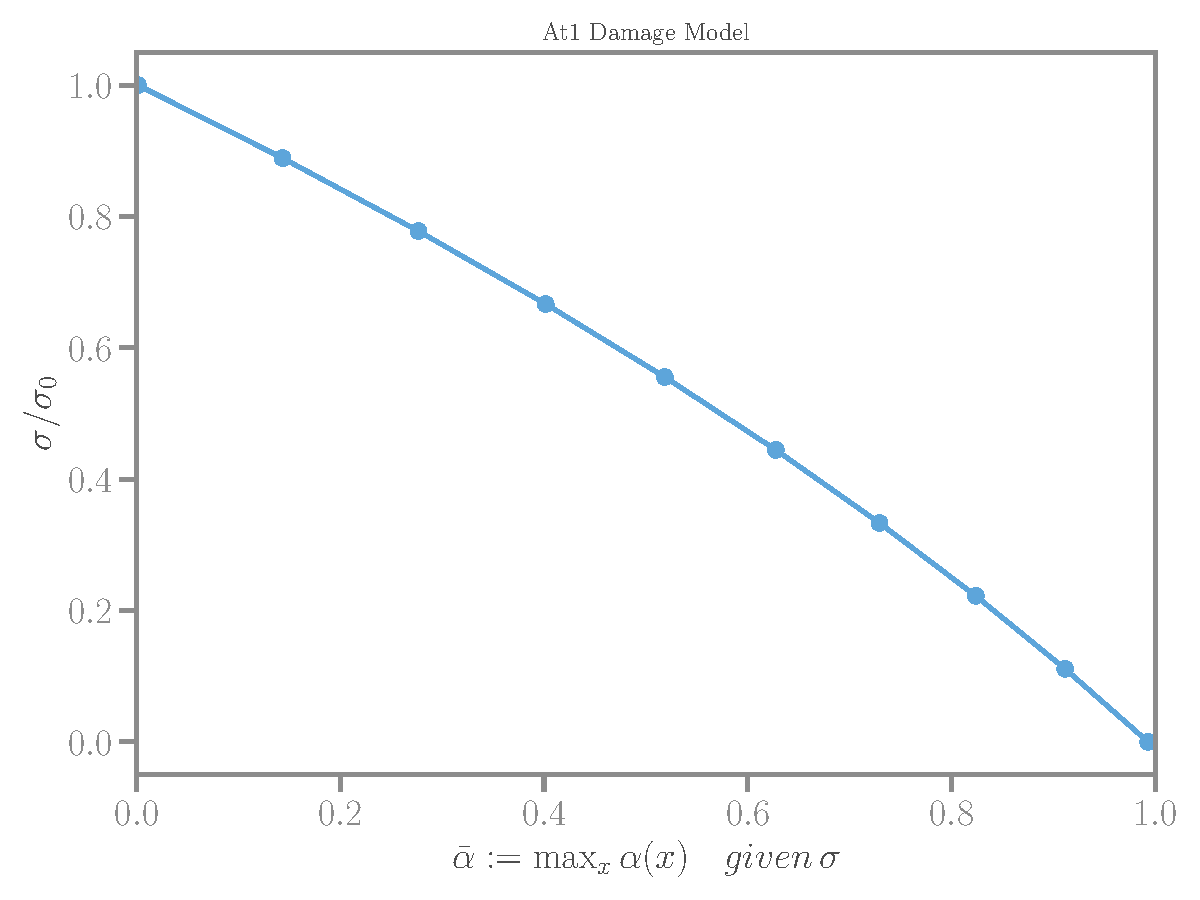
\includegraphics[width=.33\textheight]{../figures/at1-maxalpha.pdf}
  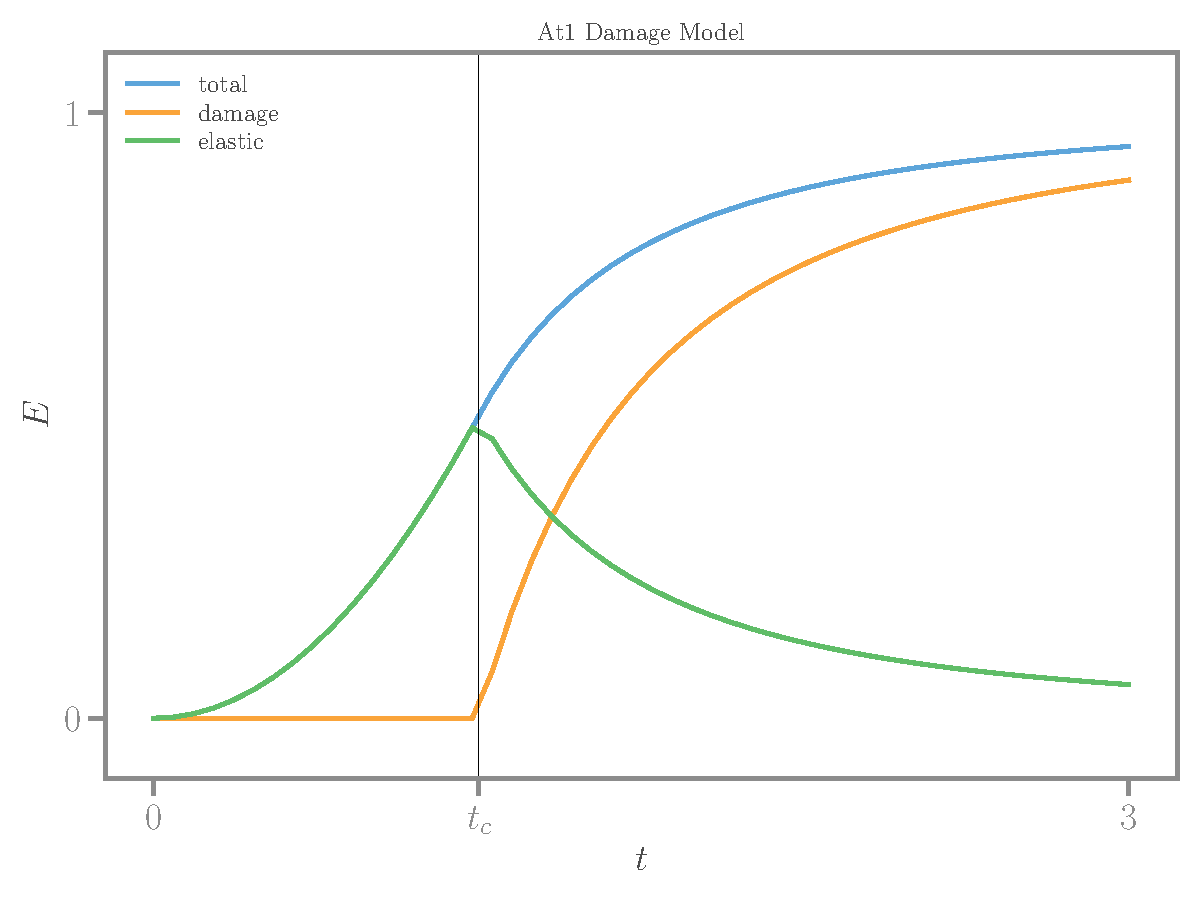
\includegraphics[width=.33\textheight]{../figures/at1-energies-homog.pdf}
  \caption{class analysis}
  \label{fig:class-analyser}
\end{figure}

\section*{PQ}

energy
\begin{equation}
  \label{eqn:mod-energy}
E(y)  =  \int_0^L
0.5 E_{0} \left(1 - \alpha{\left(x \right)}\right)^{q} \left(\alpha{\left(x \right)} + 1\right)^{- p} \left(\frac{d}{d x} u{\left(x \right)}\right)^{2} + w_{1} \left(\ilen^{2} \left(\frac{d}{d x} \alpha{\left(x \right)}\right)^{2} + \frac{\sigma_c^{2} \left(p + q\right) \alpha{\left(x \right)}}{E_{0}}\right)\end{equation}


parameters
$p, q, E_0, L, w_1, \ilen, \sigma_c $

criterion
\begin{equation}
  \label{eqn:mod-criterion}
  0=
\left(p + q\right) \left(- \frac{ E_{0}^{2} t^{2}}{2L^{2}} + w_{1} \sigma_c^{2}\right)
\end{equation}



\begin{figure}[htbp]
  \centering
  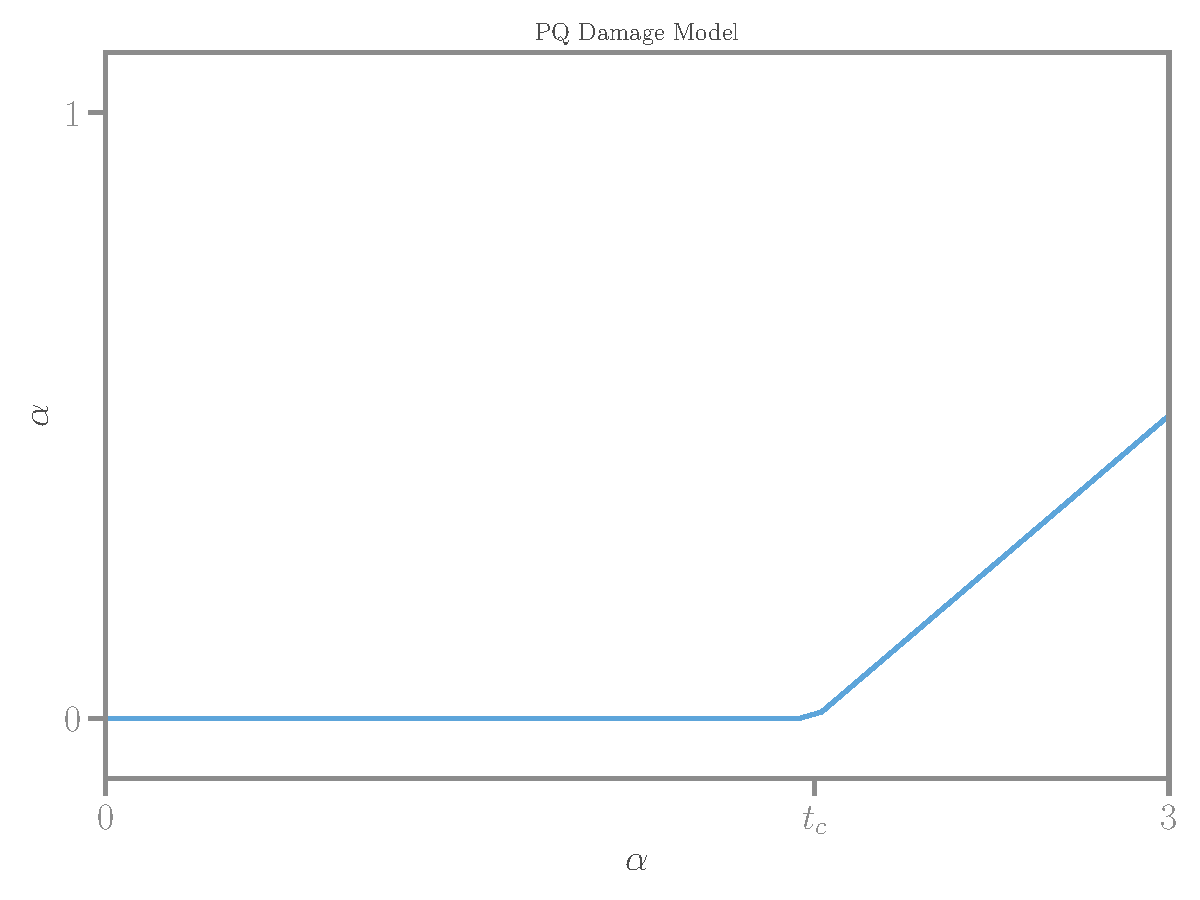
\includegraphics[width=.33\textheight]{../figures/pq-alpha-homog.pdf}
  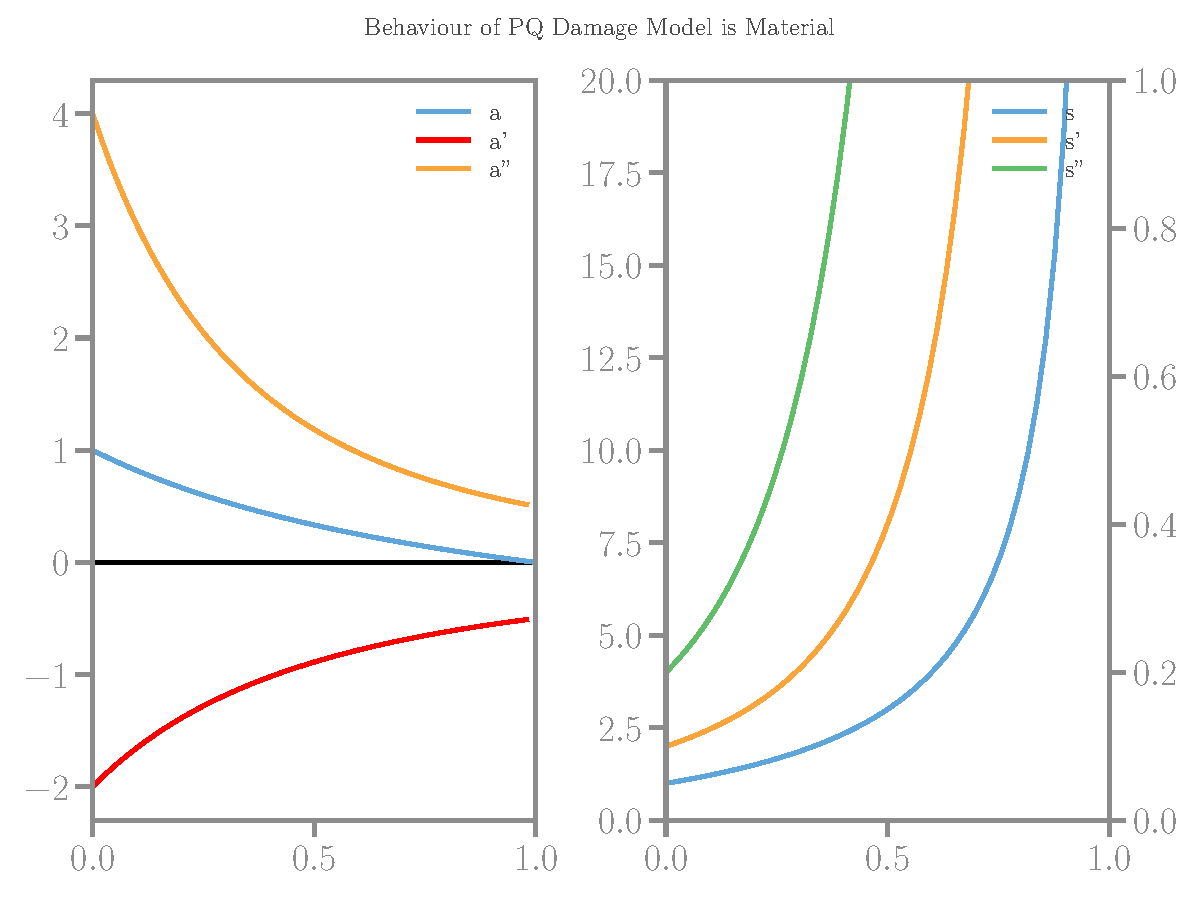
\includegraphics[width=.33\textheight]{../figures/pq-11-model.pdf}
  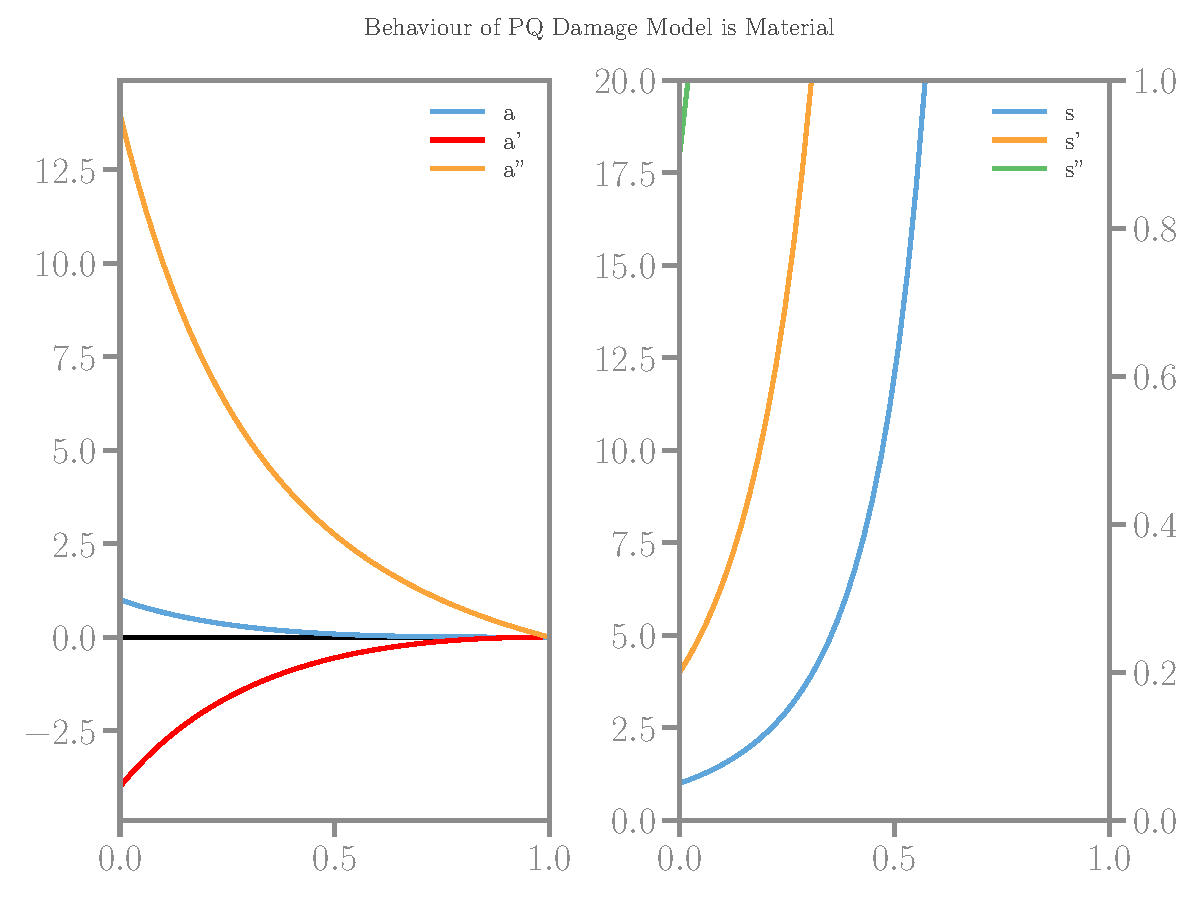
\includegraphics[width=.33\textheight]{../figures/pq-13-model.pdf}
  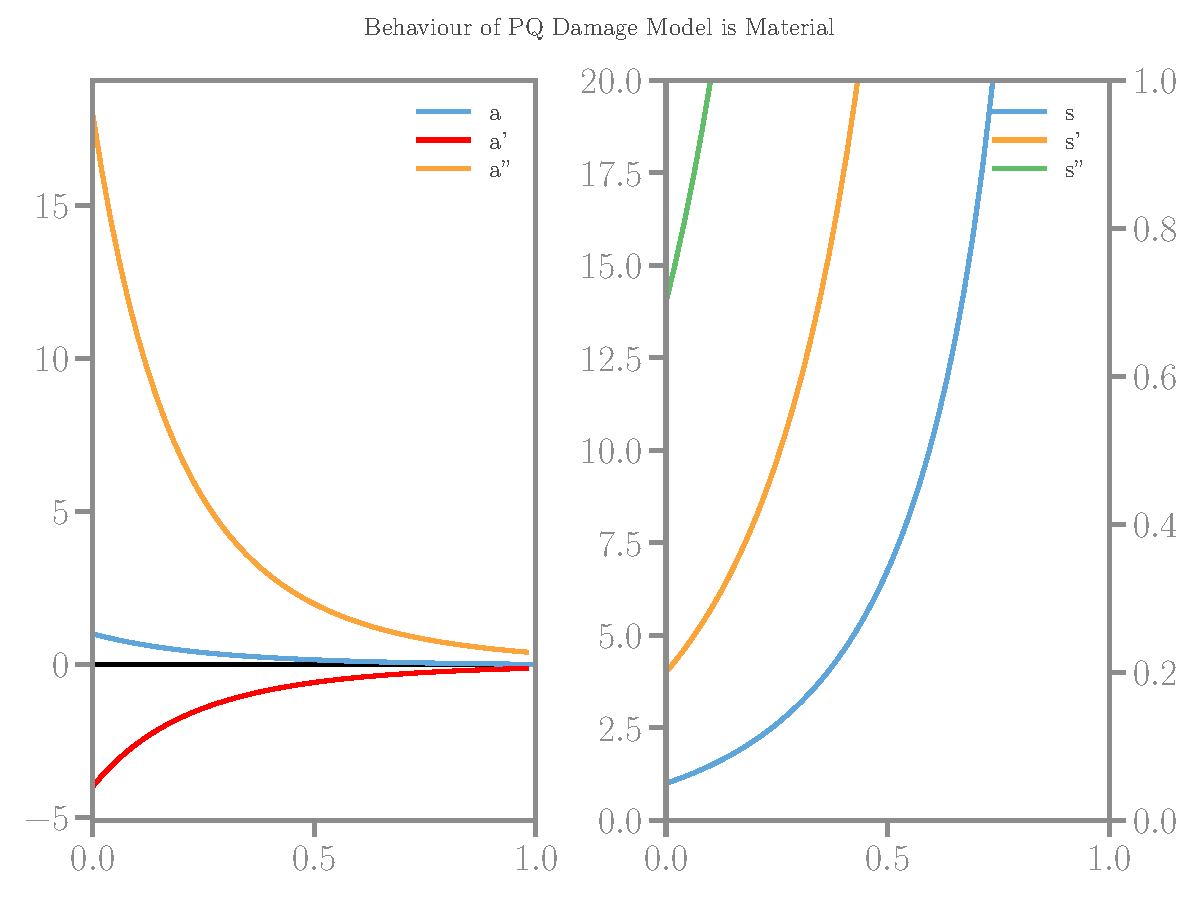
\includegraphics[width=.33\textheight]{../figures/pq-31-model.pdf}
  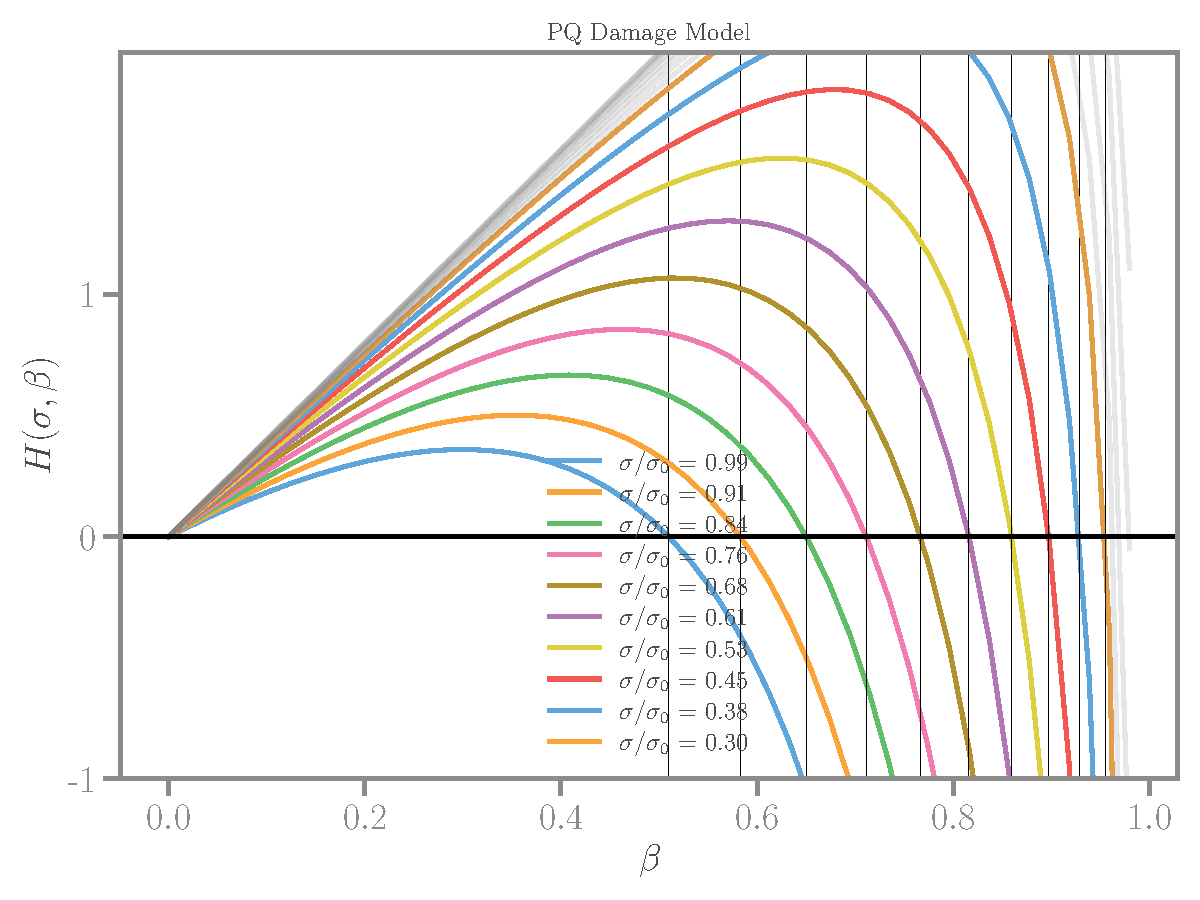
\includegraphics[width=.33\textheight]{../figures/pq-Hbeta.pdf}
  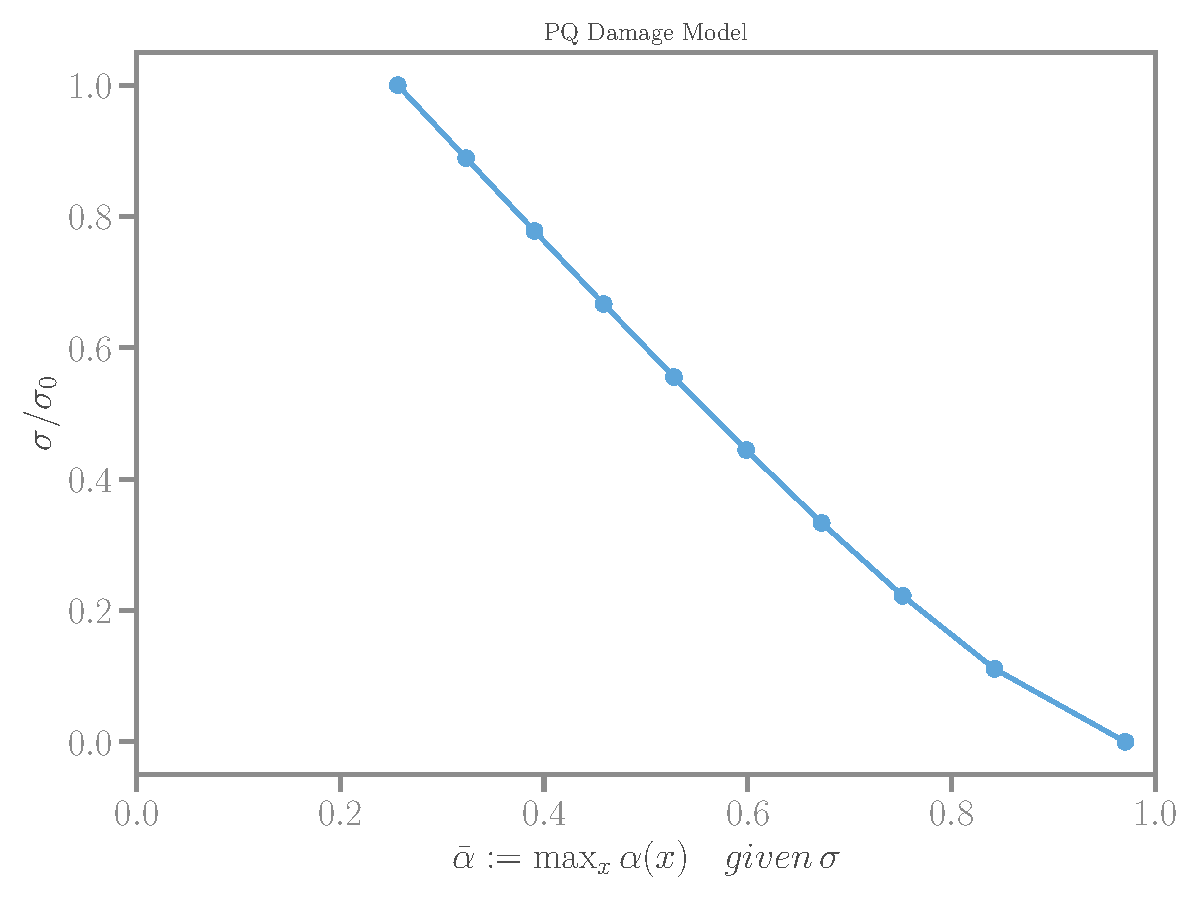
\includegraphics[width=.33\textheight]{../figures/pq-maxalpha.pdf}
  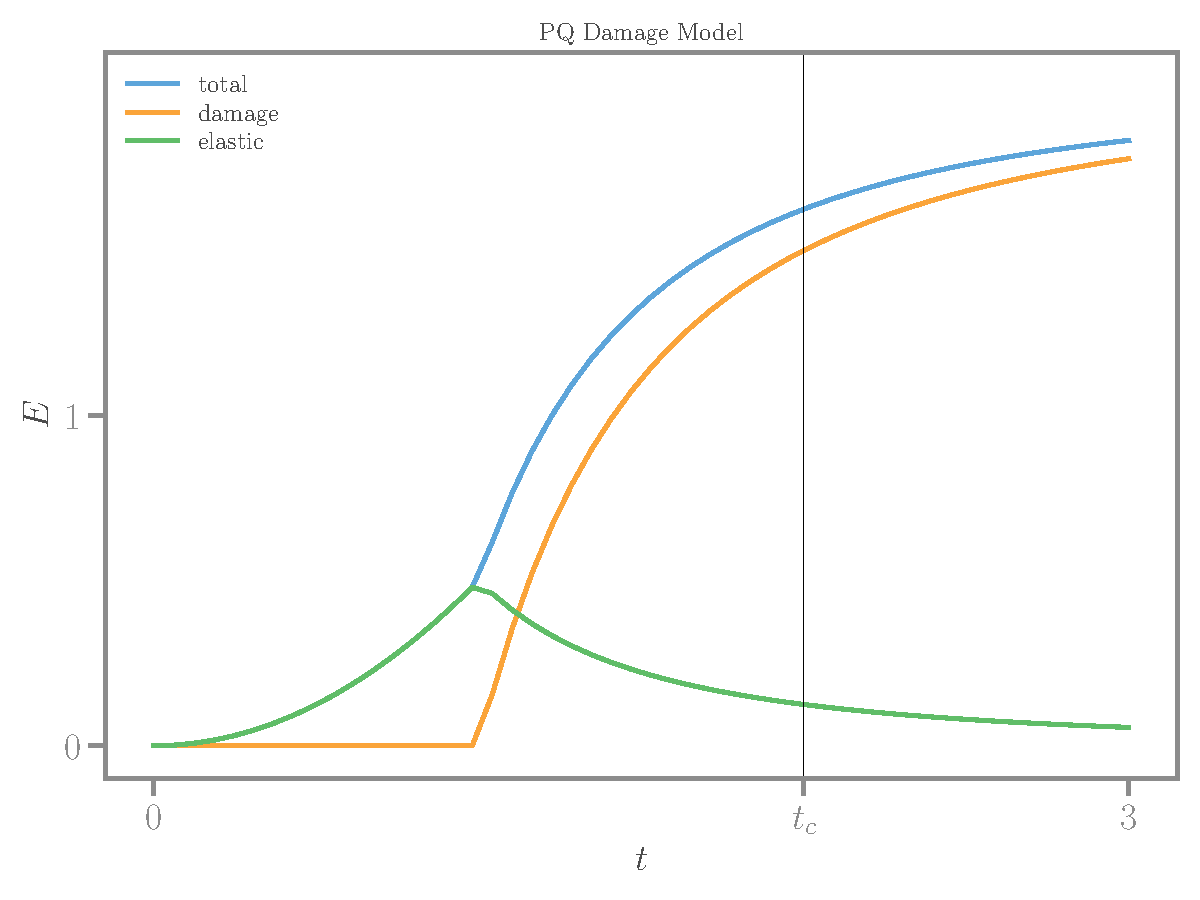
\includegraphics[width=.33\textheight]{../figures/pq-energies-homog.pdf}
  \caption{class analysis}
  \label{fig:class-analyser}
\end{figure}


\subsection*{$p=q=1$}

$$
a_t = 0.5 t - 1.0
$$
\subsection*{$p=1, q=2$}
\subsection*{$p=2, q=1$}
\end{document}

